\chapter{Revis\~ao Bibliogr\'afica}
\label{chap:revbib}

% Trecho extraído do modelo http://www2.dainf.ct.utfpr.edu.br/ppgca/estrutura-academica/regulamentacao/avaliacao/copy_of_ModeloProjetoeSeminarios.doc/view
Neste capítulo estará a sustentação teórica do trabalho, deverá ser abordado:
O conhecimento divulgado sobre o problema.
Os estudiosos do problema e os respectivos enfoques.
As diversas posições sobre o problema, suas convergências e divergências.
Indicação dos conceitos adotados para o presente estudo.
Toda a fundamentação teórica do trabalho estará nesse capítulo.
Como o programa é interdisciplinar, é comum existir mais de uma área envolvida para a revisão bibliográfica, sendo no mínimo duas: saúde e tecnologia. Após a apresentação do tema e dos assuntos pertinentes a cada uma das áreas, deve ser feita uma finalização integrando as áreas abordadas.
A revisão bibliográfica deverá conter artigos de periódicos nacionais e internacionais, para que se obtenha uma visão ampliada sobre o assunto. A maior parte da revisão bibliográfica deverá ser baseada em artigos de periódicos, considerando-se a dinamicidade e atualidade dos mesmos. 
Devem ser definidos e conceituados todos os termos significativos do trabalho. Dependendo das características do trabalho, pode-se realizar uma rápida revisão histórica, lembrando dos grandes nomes das áreas em questão e citando os trabalhos pioneiros. Uma busca ampla, e que contemple as áreas envolvidas, dará embasamento ao trabalho e segurança para o seu desenvolvimento. Assim, a revisão bibliográfica é o primeiro grande passo de qualquer trabalho científico.
A utilização dos trabalhos da revisão bibliográfica deverá preservar respeito à posição dos autores. O trabalho deverá discutir a posição dos autores, tentando avançar o estado da arte.

\section{Como utilizar ilustra\c{c}\~{o}es}

A legenda das ilustrações deve vir abaixo da mesma (ver figura \ref{fig:cliente-servidor}  e quadro \ref{tab:sus} ). 

\begin{figure}[htbp]
	\centering
	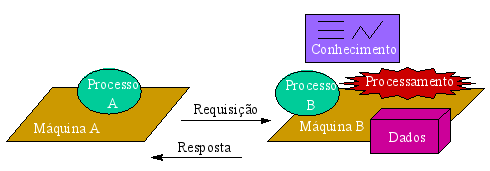
\includegraphics[width=0.9\textwidth]{./imagens/diagrama-cliente-servidor.png} % <- formatos PNG, JPG e PDF
	\caption[Paradigma Cliente-Servidor]{Paradigma Cliente-Servidor - Dados}
	\fonte{\cite{DBL98}}
	\label{fig:cliente-servidor}
\end{figure}

\begin{table}[htbp]
	\caption{Sistemas de Informação de Saúde do SUS}
	\label{tab:sus}
	\begin{tabular}{|p{4cm}|p{2.5cm}|p{4cm}|p{4cm}|}
		\hline
		SISTEMAS & EVENTO & INSTRUMENTO DE COLETA & UTILIZAÇÃO \\ \hline
		SIM - Sistema de Informações sobre Mortalidade & Óbito & Declaração de Óbito & Estudos de mortalidade, vigilância de óbitos (infantil, materno). \\ \hline
		SINASC - Sistema de Informações sobre Nascidos Vivos & Nascido Vivo & Declaração de Nascido Vivo & Monitoramento da saúde da criança, vigilância da criança de risco. \\ \hline
		SINAN - Sistema de Informações de Agravos Notificáveis & Agravos Sob Notificação & Fichas Individuais de Notificação e Investigação & Acompanhamento dos agravos sob notificação, surtos, epidemias. \\ \hline
		SIH - Sistema de Informações Hospitalares & Informação Hospitalar & Autorização de Internação Hospitalar & Morbidade hospitalar, gestão hospitalar, custeio da atenção hospitalar. \\ \hline
		SAI - Sistema de Informações Ambulatorial & Produção Ambulatorial & Boletim de Produção Ambulatorial & Acompanhamento da produção ambulatorial, gestão Ambulatorial custeio da atenção ambulatorial. \\ \hline
		SISVAN - Sistema de Vigilância Alimentar e Nutricional & Estado Nutricional & Cartão da Criança e Cartão da Gestante & Estado nutricional de crianças de zero a cinco anos e gestantes. \\ \hline
		API - Avaliação do Programa de Imunizações & Vacinas Aplicadas & Boletim Mensal de Doses Aplicadas & Contém informações referentes às doses de vacinas aplicadas. \\ \hline
	\end{tabular}
	\fonte{\cite{sus2001}}
\end{table}
%-------------------------------------------------------------------------------


A seguir ilustra-se a forma de incluir figuras, tabelas, equa\c{c}\~oes, siglas e s\'imbolos no documento, obtendo indexa\c{c}\~ao autom\'atica em suas respectivas listas. A numera\c{c}\~ao sequencial de figuras, tabelas e equa\c{c}\~oes ocorre de modo autom\'atico. Refer\^encias cruzadas s\~ao obtidas atrav\'es dos comandos {\ttfamily \textbackslash label\{\}} e {\ttfamily \textbackslash ref\{\}}. Por exemplo, n\~ao \'e necess\'ario saber que o n\'umero deste cap\'itulo \'e~\ref{chap:revbib} para colocar o seu n\'umero no texto. Isto facilita muito a inser\c{c}\~ao, remo\c{c}\~ao ou reloca\c{c}\~ao de elementos numerados no texto (fato corriqueiro na escrita e corre\c{c}\~ao de um documento acad\^emico) sem a necessidade de renumer\'a-los todos.

\section{Figuras}

Na figura~\ref{fig:dummy} \'e apresentado um exemplo de gr\'afico flutuante. Esta figura aparece automaticamente na lista de figuras. Para uso avan\c{c}ado de gr\'aficos no \LaTeX, recomenda-se a consulta de literatura especializada~\cite{Goossens2007}.


\begin{figure}[!htb]
	\centering
	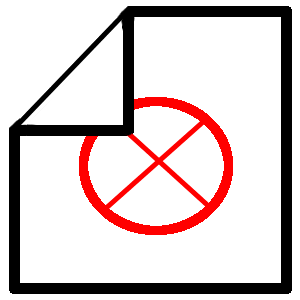
\includegraphics[width=0.2\textwidth]{./imagens/dummy.png} % <- formatos PNG, JPG e PDF
	\caption[Exemplo de uma figura]{Exemplo de uma figura onde aparece uma imagem sem nenhum significado especial.}
	\fonte{\cite{abnTeX2009}}
	\label{fig:dummy}
\end{figure}


\section{Tabelas}

% Trecho extraído do modelo http://www2.dainf.ct.utfpr.edu.br/ppgca/estrutura-academica/regulamentacao/avaliacao/copy_of_ModeloProjetoeSeminarios.doc/view
O título de uma tabela deve estar acima da mesma (ver tabela \ref{tab:patologias}).

\begin{table}[htbp]
	\centering
	\caption{Percentual das patologias identificadas nos prontuários analisados de 2003 a 2005}
	\label{tab:patologias}
	\begin{tabular}{|c|c|}
		\hline
		PATOLOGIAS IDENTIFICADAS & PERCENTUAL (\%) \\ \hline
		Lesão sobre o Nervo Femoral & 3,40\% \\ \hline
		Espondilolistese Lombar & 7,90\% \\ \hline
		Encurtamento Muscular Lombar & 9,60\% \\ \hline
		Alteração Muscular em MMII & 17,50\% \\ \hline
		Comprometimento Sacro-Ilíaca & 2,80\% \\ \hline
		Disfunção Neurológica Radicular Cervical & 9,00\% \\ \hline
		Síndrome do Desfiladeiro Torácico & 2,30\% \\ \hline
		Lombalgia & 27,70\% \\ \hline
		Cervicalgia & 19,80\% \\ \hline
	\end{tabular}
	\fonte{\cite{LAP05}}
\end{table}

%-------------------------------------------------------------------------------

Tamb\'em \'e apresentado o exemplo da tabela~\ref{tab:correlacao}, que aparece automaticamente na lista de tabelas. Informa\c{c}\~oes sobre a constru\c{c}\~ao de tabelas no \LaTeX\ podem ser encontradas na literatura especializada~\cite{Lamport1986,Buerger1989,Kopka2003,Mittelbach2004}.

\begin{table}[!htb]
	\centering
	\caption[Exemplo de uma tabela]{Exemplo de uma tabela mostrando a correla\c{c}\~ao entre x e y.}
	\label{tab:correlacao}
	\begin{tabular}{cc}
		\hline 
		x & y \\
		\hline
		1 & 2 \\
		3 & 4 \\
		5 & 6 \\
		7 & 8 \\
		\hline 
	\end{tabular}
	\fonte{Autoria pr\'opria.}
\end{table}

\section{Equa\c{c}\~oes}

A transformada de Laplace \'e dada na equa\c{c}\~ao~(\ref{eq:laplace}), enquanto a equa\c{c}\~ao~(\ref{eq:dft}) apresenta a formula\c{c}\~ao da transformada discreta de Fourier bidimensional\footnote{Deve-se reparar na formata\c{c}\~ao esteticamente perfeita destas equa\c{c}\~oes!}.

\begin{equation}
X(s) = \int\limits_{t = -\infty}^{\infty} x(t) \, \text{e}^{-st} \, dt
\label{eq:laplace}
\end{equation}

\begin{equation}
F(u, v) = \sum_{m = 0}^{M - 1} \sum_{n = 0}^{N - 1} f(m, n) \exp \left[ -j 2 \pi \left( \frac{u m}{M} + \frac{v n}{N} \right) \right]
\label{eq:dft}
\end{equation}

\section{Siglas e s\'imbolos}

O pacote \textsc{abn}\TeX\ permite ainda a defini\c{c}\~ao de siglas e s\'imbolos com indexa\c{c}\~ao autom\'atica atrav\'es dos comandos {\ttfamily \textbackslash sigla\{\}\{\}} e {\ttfamily \textbackslash simbolo\{\}\{\}}. Por exemplo, o significado das siglas\sigla{CPGEI}{Programa de P\'os-gradua\c{c}\~ao em Engenharia El\'etrica e Inform\'atica Industrial},\sigla{DAELN}{Departamento Acad\^emico de Eletr\^onica} e\sigla{UTFPR}{Universidade Tecnol\'ogica Federal do Paran\'a} aparecem automaticamente na lista de siglas, bem como o significado dos s\'imbolos\simbolo{$\lambda$}{comprimento de onda},\simbolo{$v$}{velocidade} e\simbolo{$f$}{frequ\^encia} aparecem automaticamente na lista de s\'imbolos. Mais detalhes sobre o uso destes e outros comandos do \textsc{abn}\TeX\ s\~ao encontrados na sua documenta\c{c}\~ao espec\'ifica~\cite{abnTeX2009}.

% Trecho extraído do modelo http://www2.dainf.ct.utfpr.edu.br/ppgca/estrutura-academica/regulamentacao/avaliacao/copy_of_ModeloProjetoeSeminarios.doc/view
Elemento opcional elaborado de acordo com a ordem apresentada no texto, seguido do significado correspondente. Caso não haja símbolos, não é necessário incluir a lista de símbolos.

Adaptação para usar comando \\simbolo{}
% Lista de símbolos matemáticos: http://web.ift.uib.no/Fysisk/Teori/KURS/WRK/TeX/symALL.html

\begin{itemize}
	\item \simbolo{$\bar{x}$}{Tempo médio de uma amostra}: Tempo médio de uma amostra.
	\item \simbolo{$\sigma$}{Desvio Padrão}: Desvio Padrão.
	\item \simbolo{$n$}{Número de valores da amostra}: Número de valores da amostra.
	\item \simbolo{$\Delta$}{Variação do intervalo de confiança de 95\% para a estimação da média da população}: Variação do intervalo de confiança de 95\% para a estimação da média da população.
\end{itemize}


%-------------------------------------------------------------------------------
